%!TeX root = MOSFET_selection
\documentclass[main.tex]{subfiles}

\begin{document}
    \section{MOSFET selection}
    \justify
    In this section, the criteria of selecting a suitable MOSFET are discussed.
    \begin{enumerate}
        \item \nameref{sec:switch_type}.
        \item \nameref{sec:on_resistance}.
        \item \nameref{sec:gate_charge}.
        \item \nameref{sec:soa}.
        \item \nameref{sec:irf4905}.
    \end{enumerate}

    \pagebreak
    \subsection{MOSFET switching principle} \label{sec:switch_type}

    \justify
    The N-channel and P-channel MOSFET have different turn-on conditions:
    \begin{itemize}
        \item For the N-channel MOSFET to be  "switched on" (in triode or saturation region), $V_{gs} > V_{th}$ with Gate-Source threshold voltage $V_{th} > 0$. To achieve this, a simple circuit such as in Figure \ref{fig:simple_nmos_switch} can be used. This configuration is called \textbf{Low-side Switch} where  the switch (MOSFET) is connected to the negative terminal of the supply voltage.
        \item For the P-channel MOSFET, the turn-on condition is $V_{gs} < V_{th}$ with $V_{th} < 0$ which leads to the simple circuit shown in Figure \ref{fig:simple_pmos_switch}. This configuration is called \textbf{High-side Switch} where the switch is connected to the positive terminal of the supply voltage.
    \end{itemize}
     

    \begin{figure}[!h]
        \centering
        \begin{minipage}{.4\textwidth}
          \centering
          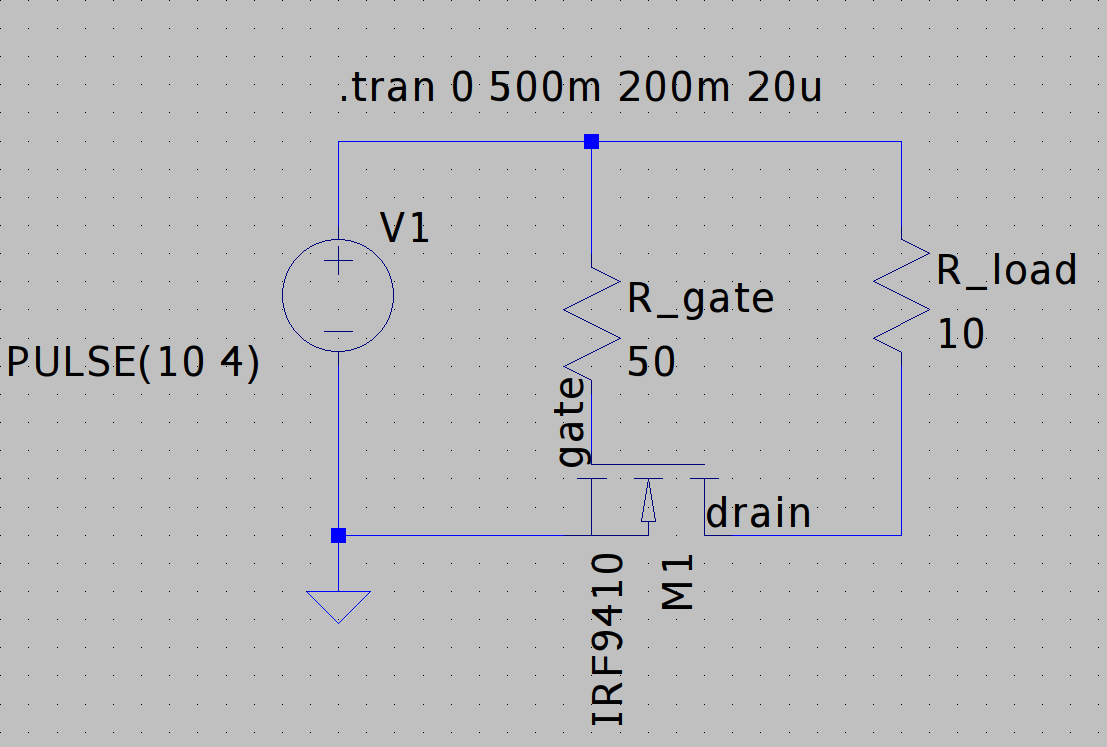
\includegraphics[width=\linewidth]{media/nmos_switch.png}
          \captionof{figure}{Low-side MOSFET switch.}
          \label{fig:simple_nmos_switch}
        \end{minipage}\qquad
        \begin{minipage}{.4\textwidth}
          \centering
          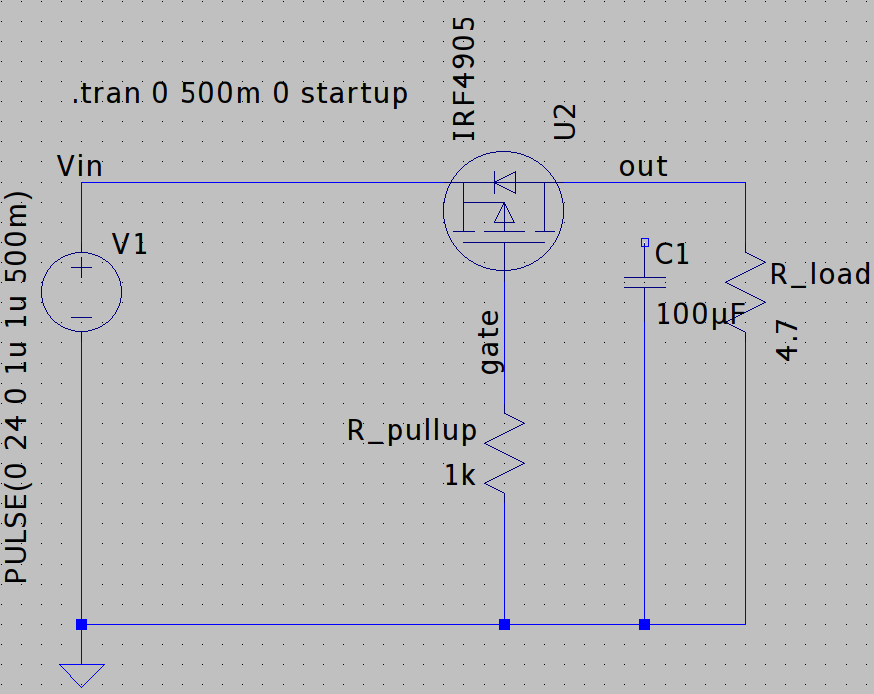
\includegraphics[width=\linewidth]{media/pmos_switch.png}
          \captionof{figure}{High-side MOSFET switch.}
          \label{fig:simple_pmos_switch}
        \end{minipage}
    \end{figure}

    \justify
    In load switching application, high-side switching is more preferable due to having no ground offset (ground loop). In a circuit exhibiting ground loop, the load is not connected directly to the ground of the power supply which can lead to distortion in signal transmission. The offset voltage is calculated by $\Delta V_\text{GND} = -I_d \cdot R_{ds}$ showing that $\Delta V_\text{GND}$ varied, and, thus, not desirable in electronics system.    

    \pagebreak
    \subsection{On resistance $R_{ds}$} \label{sec:on_resistance}
    N-channel MOSFET exhibits lower $R_{ds}$ than that of P-channel MOSFET due to packing density. It is possible to parallel two or more P-channel MOSFETs to reduce the total on resistance $R_{\sum ds}$. However, the designer has to take into account devices' parameters mismatch. An application note from Infineon and Texas Instruments \cite{InfineonParallelMOS} details the effects and solutions of each mismatches, suitable for paralleling up to 4 MOSFETs. However, \cite{MOSFET_parallel_low_power} shows that for low power application, the parameter mismatches is not as detrimental as for high power application.
    
    \pagebreak
    \subsection{Gate Charge} \label{sec:gate_charge}

    \justify
    For a MOSFET to be switched-on, the parasitic capacitors $C_{gs}$ and $C_{gd}$ modeled in Figure \ref{fig:MOSFET_parasitic_cap} has to be charged/discharged. This phenomenon is synonymous to both P-channel and N-channel MOSFET. Thus, in this section, the gate charge curve of P-channel MOSFET is discussed.

    \begin{figure}[!h]
        \centering
        \begin{minipage}{.5\textwidth}
          \centering
          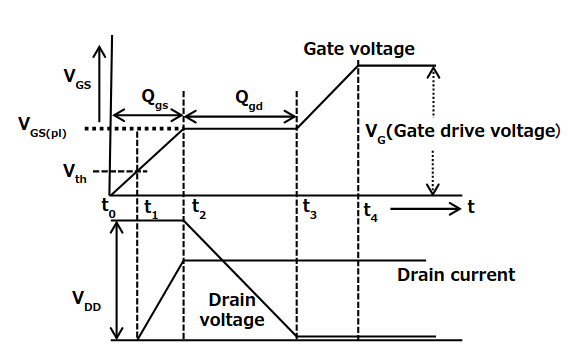
\includegraphics[width=\linewidth]{media/gate_charge_curve_details.png}
          \captionof{figure}{Typical gate charge curve.}
          \label{fig:gate_charge_curve_details}
        \end{minipage}%
        \begin{minipage}{.5\textwidth}
          \centering
          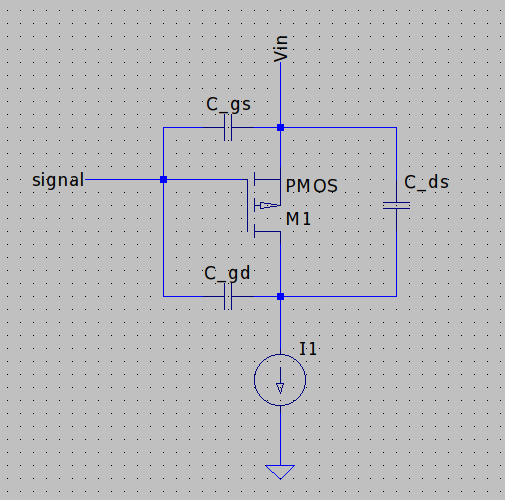
\includegraphics[width=0.8\linewidth]{media/MOSFET_parasitic_cap.png}
          \captionof{figure}{MOSFET parasitic capacitance.}
          \label{fig:MOSFET_parasitic_cap}
        \end{minipage}
    \end{figure}
    
    \justify
    During a turn-on event, it can be divided into four main intervals. These intervals are shown in Figure \ref{fig:gate_charge_curve_details}.
    \begin{enumerate}
        \item $t_0 \rightarrow t_1$: $V_{gs}$ drops to approximately $V_{th}$. At this voltage, the MOSFET enters its ohmic/linear region and starts to conduct $I_d$.
        \item $t_1 \rightarrow t_2$: $V_{gs}$ drops to $V_{gs,miller}$, \textbf{Miller plateau}. At this voltage, the MOSFET is still in its linear region. The charging time and the charge is defined by:
        \begin{equation}
            \Delta t_{0\rightarrow2}=R_{g}(C_{gs} +C_{gd})ln\left(\dfrac{V_{signal-source}}{V_{gs, miller}}\right)
        \end{equation}
        \begin{equation}
            Q_{0\rightarrow2}=(C_{gs} +C_{gd})\cdot (-V_{gs, miller})
        \end{equation}
        \item $t_2 \rightarrow t_3$: While $V_{gs}$ maintains at $V_{gs,miller}$, $V_{ds}$ starts to increases to its turn-on voltage $R_{ds}(on)\cdot I_d$ of a few $mV$, and the MOSFET enters its saturation region. Because only $V_{ds}$ decreases, $C_{gd}$ is being charged with a constant current flowing through $R_{g}$. Thus, the following equation: 
        \begin{equation}
            \dfrac{\delta V_{ds}}{\delta t}=\dfrac{1}{C_{gd}}\cdot\dfrac{V_{signal-source} - V_{gs,miller}}{R_{g}} \Rightarrow \Delta V_{ds} = \dfrac{V_{signal-source} - V_{gs,miller}}{R_{g}C_{gd}}\cdot \Delta t_{2\rightarrow3}
        \end{equation}
        \begin{equation}
            Q_{2\rightarrow3}= \left| \dfrac{V_{signal-source} - V_{gs,miller}}{R_{g}} \right|\cdot \Delta t_{2\rightarrow3} 
        \end{equation}
        Ideally, in saturation region, $V_{ds} = 0V \Rightarrow \Delta V_{d} = -V_{in}$. Therefore:
        \begin{equation}
            \Delta t_{2\rightarrow3}=\dfrac{V_{signal-source}}{V_{signal-source} - V_{gs,miller}}\cdot R_{g}C_{gd}
        \end{equation}
        \begin{equation}
            Q_{2\rightarrow3}= -V_{signal-source}\cdot C_{gd}
        \end{equation}
        
        \item $t_3 \rightarrow t_4$: In the saturation region, $V_{gs}$ starts increasing to $V_{signal}$. However, $V_{gs}$ is clamped at $D1$'s zener voltage. 
    \end{enumerate}

    \justify
    In this project's application, which does not involve high speed switching, only the interval $t_0 \rightarrow t_3$ is concerned (from turn-off and saturation region). Thus, the total turn-on time $T_{on}$ and turn-on charge $Q_{on}$ is:

    \begin{equation} 
        T_{on} = R_{g}(C_{gs} +C_{gd})ln\left(\dfrac{V_{signal-source}}{V_{gs, miller}}\right) + \dfrac{V_{signal-source}}{V_{gs,miller}}R_{g}C_{gd}
    \end{equation}

    \begin{equation} \label{eq:estimated_on_charge_1}
        Q_{on} = -[(C_{gs} +C_{gd})\cdot V_{gs, miller} - V_{signal-source}\cdot C_{gd}]
    \end{equation}

    \justify
    In a MOSFET datasheet, the value of $C_{gs}$ and $C_{gd}$ are shown in terms of input capacitance $C_{iss}$ and reverse transfer capacitance $C_{rss}$ which are plotted in the datasheet such as Figure \ref{fig:typical_capacitance_plot}. The differnce between $C_{iss}$ and $C_{rss}$ are approximately constant, meaning $C_{gs}$ is constant, while $C_{gd}$ is non-linear and dependent of $V_{in}$. $V_{gs,miller}$ can be estimated by \eqref{eq:estimated_miller_voltage_TI} with $V_{th}$ and $K_n$ are unique to each MOSFET. Finally, \eqref{eq:estimated_on_charge_1} can be rewritten in \eqref{eq:estimated_on_charge_2}.

    \begin{figure}[!h]
        \centerline{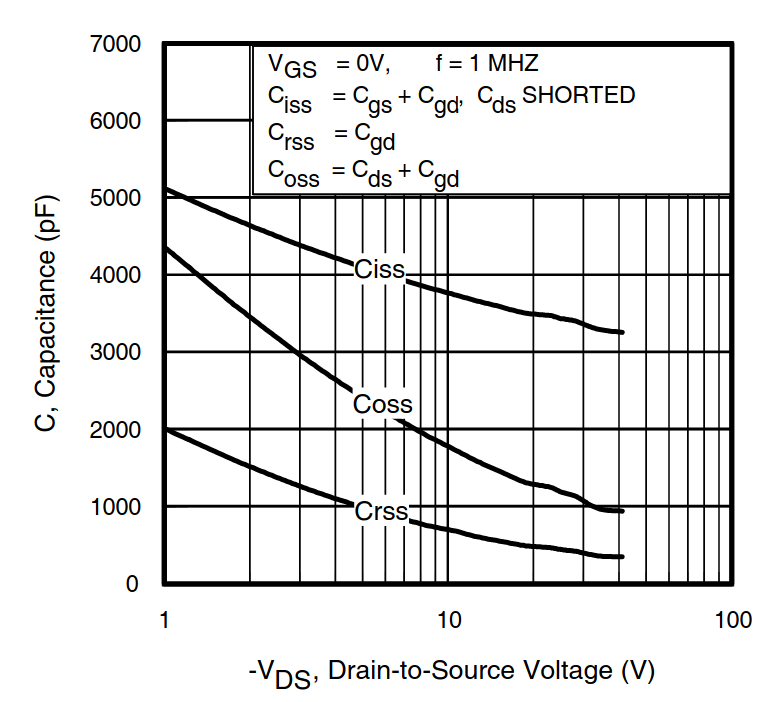
\includegraphics[scale=0.25]{media/typical_capacitance_plot.png}}
        \caption{Typical capacitance vs. Drain-Source voltage.}
        \label{fig:typical_capacitance_plot}
    \end{figure}

    \begin{equation} \label{eq:estimated_miller_voltage_TI}
        V_{gs, miller} = V_{th} + \sqrt{\frac{I_{d}(\infty)}{K_n}}
    \end{equation}

    \begin{equation} \label{eq:estimated_on_charge_2}
        Q_{on} = [C_{gs} +C_{gd}(V_{in})]\cdot \left(V_{th} + \sqrt{\dfrac{I_{d}(\infty)}{K_n}} \right) + V_{signal-source}\cdot C_{gd}(V_{in})
    \end{equation}

    \justify
    For quick prototyping, the total gate charge $Q_g$ in the MOSFET's datasheet can be used. In the case of IRF4905S, $Q_g$ is $180nC$. For a charge/discharge time of, e.g.,  $t_{sw} = 100ns$, the gate current to switch the MOSFET can be approximated as $I_g = Q_g / t_{sw} = 1.8A$.

    \pagebreak
    \subsection{Safe Operating Area (SOA)} \label{sec:soa}
    In a MOSFET's datasheet, the SOA of the device shows the limitation of the device's opreating range. As long as the desired application is well within the SOA, the device will, in all likelihood, not risk running into problems such as thermal runaway, material degradation, etc. A typical SOA plot of a P-channel MOSFET is shown in figure \ref{fig:typical_SOA_plot}. The SOA lies below the dashed boundary.

    \begin{figure}[!h]
        \centering
        \begin{minipage}{.5\textwidth}
          \centering
          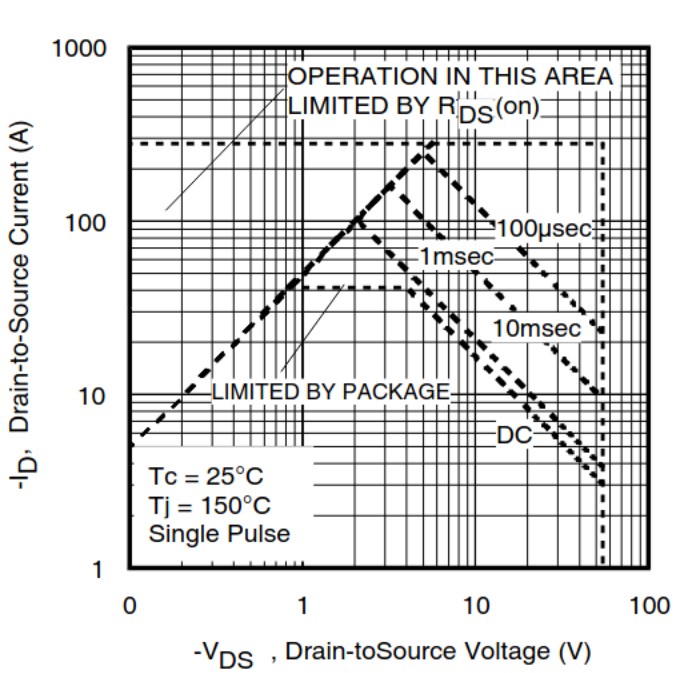
\includegraphics[width=0.8\linewidth]{media/typical_SOA_plot.png}
          \captionof{figure}{Typical MOSFET's SOA plot.}
          \label{fig:typical_SOA_plot}
        \end{minipage}%
        \begin{minipage}{.5\textwidth}
          \centering
          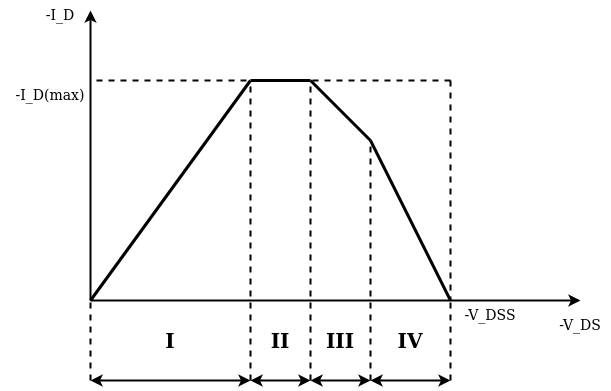
\includegraphics[width=\linewidth]{media/SOA_regions.drawio.png}
          \caption{Regions within a MOSFET's SOA.}
        \label{fig:SOA_regions}
        \end{minipage}
    \end{figure}

    \justify
    The SOA can be divided into four regions shown in figure \ref{fig:SOA_regions}:
    \begin{enumerate}
        \item Region I:$-V_{ds}$ is determined purely by Ohm's law  $-V_{ds} = R_{ds}(\text{on})\cdot -I_d$ with $-I_d \leq -I_{d,\text{max}}$. Thus, region I spans from $-V_{ds} = 0$ to $-V_{ds} = \dfrac{-I_{d,\text{max}}}{R_{ds}(\text{on})}$.
        \item Region II: $-I_{d}$ is limited by $-I_{d,\text{max}}$ as a result of limitation of package, silicon and junction-to-ambient thermal impedance $R_{\theta J A}$. The power consumption $P=I_{d} * V_{ds}$ does not exceed the maximum rating. Thus, region II spans from $-V_{ds} = -I_{d,\text{max}} / R_{ds}(\text{on})$ to $-V_{ds} = \dfrac{P_\text{max}}{-I_{d,\text{max}}}$.
        \item Region III: the $-I_{d}$ is limited by $P_\text{max}$ or $-I_d = \dfrac{P_\text{max}}{-V_{ds}}$, hence, the negative coefficient observed from the plot.
        \item Region IV: The forth region is limited by thermal instability. 
    \end{enumerate}

    \justify
    Texas Instruments \cite{TISOA} noted the following:
    \begin{itemize}
        \item Region III's and IV's boundary mostly unanimous. Hence, the application should be designed to operate well within the estimated regions defined in the datasheet. 
        \item Besides region I, the other regions are soft-limited, meaning that operation outside of these regions does not guarantee immediate damage. However, the longevity of the devie is affected.
    \end{itemize}

    \justify
    To ensure the operation of the MOSFET is well within the SOA, the following basic parameters of the device should be:

    \begin{enumerate}
        \item Drain-Source breakdown voltage $V_{dss}$ is at least 20\% higher than the operating voltage. 
        \item Maximum continuous Drain current $I_{d,\text{max}}$ is at least 20\% higher than the operating current.
        \item Low on resistance $R_{ds}$ satisfying the maximum dissipation power $P_{d}=R_{ds} \cdot I_{max}$ of the MOSFET.
    \end{enumerate}

    \pagebreak
    \subsection{IRF4905S} \label{sec:irf4905}

    \justify
    As a load switch, the following parameters are basic to the selection process:
    \begin{itemize}
        \item Safe Operating Area is guaranteed.
        \item Parsitic capacitance $C_{gd}$ does not vary largely over the operating range.
    \end{itemize}

    \justify
    Between N-channel and P-channel MOSFET, within the same price range, $V_{ds}$ and $I_d$ are similar. The main differences are the switch type (high-side or low-side) and the $R_{ds}$. These differences are discussed in details in previous sections, and is summarized in Table \ref{table:MOSFET_channel_type}
    

    \begin{table}[!h]
        \centering
        \begin{tabular}{|m{0.15\linewidth}|m{0.4\linewidth}|m{0.4\linewidth}|}
        
        \hline
        & \textbf{P-channel MOSFET} &  \textbf{N-channel MOSFET} \\
        \hline
        \textbf{Switch type} & $V_{th} < 0V \Rightarrow$ High-side switch & 
        \begin{itemize}
            \item $V_{th} > 0V \Rightarrow $ Low-side switch leads to ground offset (ground loop) varied based on $R_{ds}$ and $I_{d}$ of MOSFET. Require a gate driver IC with integrated/discrete charge pump circuit to use as high-side switch.
        \end{itemize}
        \\
        \hline
        \textbf{Typical $R_{ds}$} & 
        \begin{itemize}
            \item High, in $100 m\ohm$ range $\Rightarrow$ High power loss. By paralleling, the on resistance is halved.
            \item Low $R_{ds}$ is more expensive than its N-channel counterpart.
        \end{itemize}
         
        & Low, in $m\ohm$ range $\Rightarrow$ Low power loss.
        \\
        
        \hline
        \end{tabular}
        \caption{Comparison of P-channel \& N-channel MOSFET}
        \label{table:MOSFET_channel_type}

    \end{table}    

    \justify
    Considering the advantages and disadvantages of the two type of MOSFET transistor, it is clear that using P-channel MOSFET as high-side switch is more advantageous in terms of components counts. Finally, the IRF4905S MOSFET is used because it has a suitable margin between its $V_{ds}$ and $I_{d}$ values and a low $R_{ds}$, making it ideal for this application. 

    \begin{figure}[!h]
        \centerline{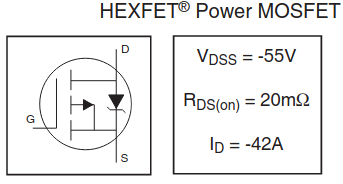
\includegraphics[scale=0.5]{media/IRF4905_key_parameters.png}}
        \caption{IRF4905 P-channel MOSFET key parameter \cite{IRF4905S}.}
        \label{fig:IRF4905S_param}
    \end{figure}    
    
\end{document}
